\chapter{Einleitung}
\label{ch:einleitung}

\section{Motivation}
\label{sec:motivation}
- Warum habe ich das gemacht?
- Was hat Bosch davon?
- Was ändert sich am Markt?
\\ \\
- Seit wann gibt es Machine Learning und seit wann wird es erst richtig genutzt
- Machine Learning ein immer Wichtigerer Aspekt im Leben
- Andere Firmen haben viel damit gemacht
- Maschinen schneller und besser einstellen können
- Maschinen Reibungsloser einstellen
- Wiederkehrende Probleme sehen
- Maschinen automatisch einstellen
- Performance der Maschine verbessern
\\ \\
Wirtschafts Woche~\cite{article_einleitung_ww_sg} und~\cite{article_einleitung_ww_cm}.
\\ \\
Deutsche Unternehmerbörse~\cite{article_einleitung_dub_ki} und~\cite{article_einleitung_dub_aw}
und~\cite{article_einleitung_dub_jb} und~\cite{article_einleitung_dub_sb} und~\cite{article_einleitung_dub_il}
\\ \\
\enquote{Intelligenz ist die Fähigkeit, sich dem Wandel anzupassen} von Stephen Hawking.
\\ \\
- Hypothese, dass ich das Problem mit Machine Learning lösen will
\\ \\
Eventuell Plakat darstellen
\\ \\
2 Seiten

\colorbox{yellow}{Hier fehlt was}

Wie in dem Comic von Dilbert\footnote{http://dilbert.com/strip/2016-06-20}.

\begin{figure}[h]
    \centering
    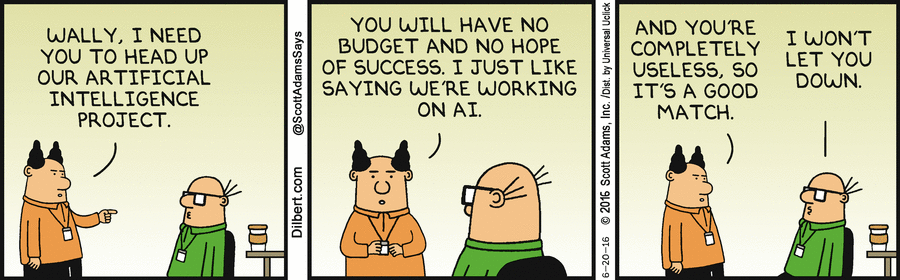
\includegraphics[width=\textwidth]{images/kapitel_1/dilbert_ai.png}
    \caption{Wie Projekte nicht ablaufen sollten}
    \label{fig:dilbert_ai}
\end{figure}

\newpage

\section{Abstract}
English Version of the motivation.
\colorbox{yellow}{Hier fehlt was}

\newpage

\section{Aufgabenstellung}
\label{sec:aufgabenstellung}
Das folgende Kapitel soll eine kleine Übersicht über die Themen geben, welche in der Arbeit behandelt werden. Für die
leichtere Umsetzung ist die Arbeit in drei größere Themenbereiche unterteilt.

Der erste Teil der Arbeit befasst sich mit dem Aufbau eines neuronalen Netzes, welches in der Cloud trainiert werden
soll. Ein Nutzer soll anschließend die Möglichkeit haben, das trainierte Netz aus der Cloud heraus zu nutzen oder es
lokal auf einem eigenen Rechner einzurichten.

Dabei sollen die Vorteile des Cloud Computings genutzt werden, um das Training eines neuronalen Netzes erheblich zu
beschleunigen. DevOps-Tools sollen dabei helfen, die Bereitstellung des Netzes und erforderliche Schnittstellen zu
vereinfachen. Cloud-Services erleichtern die Entwicklung indem sie das schreiben von Quellcode eindämmen.

Im zweiten Teil der Arbeit wird das bereitgestellte neuronale Netz über ein Frontend angesteuert um Daten zu übergeben
und die resultierenden Vorhersagen zu veranschaulichen. Ebenfalls sollen Smartphone-Apps für Android und iOS entstehen,
um die Nutzung der Anwendung im Bereich der Maschinenauslieferung zu vereinfachen.

Diverse Tests sollen die Funktionsweise des erstellten neuronalen Netzes, der Schnittstellen und des Frontends
sowie den Smartphone-Apps sicherstellen.

Der letzte Teil widmet sich der Adaptierbarkeit auf weitere Systeme, Maschinen und Netze der aufgebauten Architektur.
Dort werden weitere Szenarios aufgezeigt, die für das automatisieren von Maschinenparametern entscheidend sein können.
Es soll eine Anleitung entstehen, die das Einbauen der neuen und zukünftigen Szenarios vereinfacht.

Zum Schluss folgt ein Ausblick mit Anregungen und Erweiterungen sowohl für die Weiterentwicklung des neuronalen Netzes
als auch für das Web-Frontend und die Smartphone-Apps. Auch sollen weitere Cloud-Services aufgezeigt werden, welche
zusätzliche Möglichkeiten bieten.

Ziel ist es der Bosch Packaging GmbH dabei zu helfen, Kundenaufträge, die das Einstellen von Maschinen oder
Maschinenkomponenten beinhalten, zu beschleunigen und so die Wartezeit für den Kunden zu minimieren. Auch soll so
Fehlern vorgebeut werden und eine Hilfestellung für neue Maschineneinsteller entstehen.

\newpage

\section{Aufbau der Arbeit}
\label{sec:aufbauDerArbeit}
Dieses Kapitel dient zur schnelleren Orientierung innerhalb der Arbeit und zeigt auf, welche Themen die jeweiligen
Kapiteln behandeln.

\begin{description}

    \item[Kapitel 2 (Grundlagen)]\hfill \\
    Dieses Kapitel erklärt die Grundlagen. Es wird zum Beispiel der Unterschied zwischen den verschiedenen Cloudanbieter
    im Bereich Machine Learning erläutert, um was es sich bei TensorFlow.js handelt und was ein WebViewer ist. Außerdem
    wird die genutzten Bosch-Maschinen kurz vorgestellt.

    \item[Kapitel 3 (Neuronales Netz)]\hfill \\
    Das dritte Kapitel erläutert die Entwicklung des Machine Learning Algorithmus in der Cloud. Dabei werden verschiedene
    Optionen für die einzelnen Teilaufgaben analysiert und im Anschluss die genutzten Programme installiert, eingerichtet
    und erläutert. Das trainierte Model wird abschließend in TensorFlow.js importiert und über einen Wrapper in einem
    Container zugänglich gemacht.

    \item[Kapitel 4 (Client)]\hfill \\
    Das vierte Kapitel setzt das in der Cloud trainierte Model voraus und implementiert dazu ein prototypisches Frontend.
    Dieses besteht aus einer Angular-Anwendung sowie zwei Smartphone-Apps. Dabei werden zu Anfang verschiedene Programme
    und Services analysiert, um diese im Anschluss zu nutzen.

    \item[Kapitel 5 (Adaptierbarkeit)]\hfill \\
    Hier werden Themen angesprochen, die für die weitere Verwendung oder Erweiterung des Machine Learning Algorithmus
    oder des Frontends, entscheidend sind. Unter anderem wird erläutert, welche Schritte notwendig sind, um neue Maschinen
    oder Komponenten in die Architektur einzubauen oder wie optimale Daten zusammengestellt werden müssen.

    \item[Kapitel 6 (Ausblick)]\hfill \\
    Wie sowohl der Machine Learning Algorithmus als auch das Frontend erweitert werden kann, zeigt dieses Kapitel auf.
    Dabei können neue Cloud-Services hinzugefügt oder auch weitere Funktionen der schon eingesetzten Services verwendet
    werden.

    \item[Kapitel 7 (Zusammenfassung)]\hfill \\
    Das letzte Kapitel enthält eine Zusammenfassung aller vorangegangenen Kapitel und ein Schlusswort.

\end{description}